\documentclass[tikz,border=3pt]{standalone}
\usepackage[T1]{fontenc}
\usepackage[utf8]{inputenc}
\usepackage[english]{babel}
\usepackage{mathptmx}
\usepackage[scaled=0.92]{helvet}
\usepackage{amsmath,amssymb,textcomp}
\usetikzlibrary{positioning,arrows.meta}
\newcommand{\us}{\textmu s}
\begin{document}
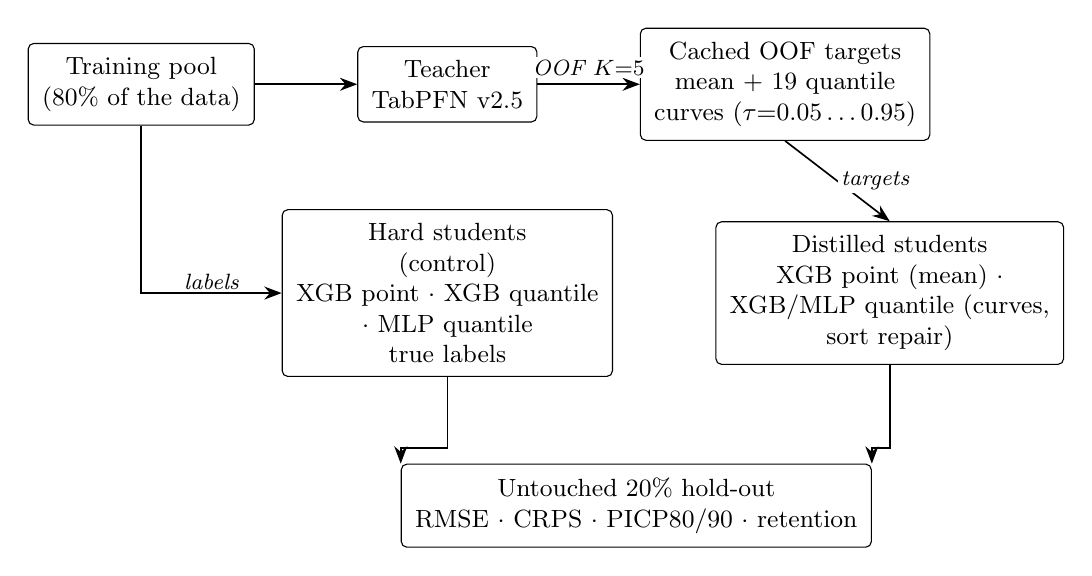
\begin{tikzpicture}[
  font=\small,
  box/.style={draw, rounded corners=2pt, align=center, inner sep=5pt,
              minimum height=9mm},
  lab/.style={font=\footnotesize\itshape, midway, fill=white, inner sep=1pt},
  arr/.style={-{Stealth[length=2.2mm]}, semithick},
  node distance=8mm and 13mm]

\node[box] (pool) {Training pool\\(80\% of the data)};
\node[box, right=of pool] (professor) {Teacher\\TabPFN v2.5};
\node[box, right=of professor] (oof) {Cached OOF targets\\mean $+$ 19 quantile\\curves ($\tau{=}0.05\,{\ldots}\,0.95$)};

\node[box, below=11mm of professor] (hard) {Hard students\\(control)\\XGB point $\cdot$ XGB quantile\\$\cdot$ MLP quantile\\true labels};
\node[box, right=of hard] (soft) {Distilled students\\XGB point (mean) $\cdot$\\XGB/MLP quantile (curves,\\sort repair)};
\node[box, below=11mm of hard, xshift=24mm] (eval) {Untouched 20\% hold-out\\RMSE $\cdot$ CRPS $\cdot$ PICP80/90 $\cdot$ retention};

\draw[arr] (pool) -- (professor);
\draw[arr] (professor) -- node[lab, above=2pt]{OOF $K{=}5$} (oof);
\draw[arr] (pool.south) |- node[lab, near end, above]{labels} (hard.west);
\draw[arr] (oof.south) -- node[lab, right]{targets} (soft.north);
\draw[arr] (hard.south) |- ([yshift=2mm]eval.north west) -- (eval.north west);
\draw[arr] (soft.south) |- ([yshift=2mm]eval.north east) -- (eval.north east);
\end{tikzpicture}
\end{document}
